Dans le modèle transitoire de stratification de bain de corium en fond de cuve de PROCOR, jusqu'à quatre couches sont considérées comme montré dans la figure \ref{fig:bain_corium_croute}. 
\begin{figure}
\centering
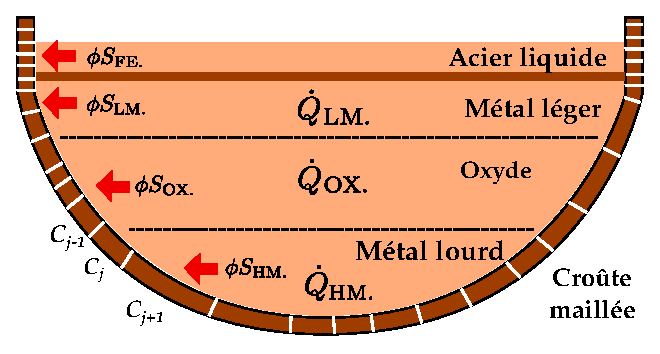
\includegraphics[width=0.7\textwidth, keepaspectratio=true]{Figures/bain_corium_croute.eps}
\caption{Bain de corium et sa croûte en fond de cuve.}
\label{fig:bain_corium_croute}
\end{figure}
De bas en haut peuvent exister une couche de métaux lourds (HM.), une couche d'oxydes (OX.) et une couche de métaux légers (LM.). Dans le modèle de stratification utilisé, la couche de métaux légers apparaît suite aux métaux remontant au travers de la couche d'oxydes lorsque le système à l'équilibre correspond à une couche de métaux légers au dessus d'une couche d'oxydes. Suivant des hypothèses de phénomènes de ségrégation de phase, ces trois couches sont entourées d'une croûte réfractaire. Une couche d'acier liquide hors équilibre (FE.), correspondant à la couche de \textit{focusing effect}, peut se trouver au dessus de ces trois couches. Seule la croûte en contact avec la cuve est modélisée dans cette note; la croûte en dessous de la couche d'acier liquide hors équilibre n'est pas modélisée par le modèle présenté et est seulement considérée en termes de fermeture pour la température entre le bain sous la croûte et cette couche. 

Les puissances résiduelles $\dot{\mathcal{Q}}$ (W) des couches métal lourd, oxyde et métal léger sont transmises, entre autres, latéralement aux mailles de la croûte sous forme de flux de chaleur $\phi S$ (W) par couche.

À l'interface entre une maille de croûte et la couche du bain correspondante, la température dépend de l'état thermique de la croûte. Si la croûte est en conduction, la température d'interface est donnée par l'égalité des flux de chaleur de part et d'autre de l'interface. Si la croûte est en fusion (resp. solidification), la température d'interface est donnée par la température de \textit{liquidus} (resp. \textit{solidus}). La température de \textit{solidus} de la croûte est donnée par la température de \textit{liquidus} de la couche de bain correspondante. Dans le modèle actuel de bain, les températures de \textit{liquidus} des trois couches de bain sous la croûte sont identiques et sont données par la température de \textit{liquidus} du bain homogène. Pour élargir le champ des possibilités, on fixera dans la note une température de \textit{liquidus} différente pour chaque couche. Pour plus de détails, voir la description du modèle de thermochimie dans la section précédente. 

Le couplage entre le modèle de bain de corium et le modèle de croûte se définit en termes d'échanges de données. De manière générale, que la croûte soit en conduction, en fusion ou en solidification, le modèle de bain de corium et le modèle de croûte échangent un flux de chaleur, une température d'interface et un débit de masse. Le couplage peut être défini sous la forme d'un graphe (voir le graphe de la figure \ref{fig:graphe_couplage_corium_croute}). 
\begin{figure}
\centering
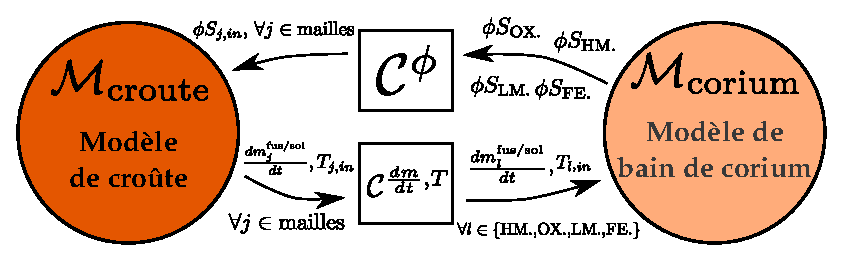
\includegraphics[width=0.7\textwidth, keepaspectratio=true]{Figures/graphe_couplage_corium_croute.eps}
\caption{Graphe du couplage entre le modèle de bain de corium et le modèle de croûte.}
\label{fig:graphe_couplage_corium_croute}
\end{figure}
Les modèles sont représentés par les n\oe{}uds du graphe et les échanges de données par des arcs entre les n\oe{}uds. Chaque arc contient un communicateur $\mathcal{C}$ permettant de faire communiquer \emph{correctement} des modèles qui, a priori, peuvent avoir des sorties et des entrées qui doivent être adaptées. Par exemple, le communicateur $\mathcal{C}^{\phi}$ permet de \emph{projeter} les puissances $\phi S$ par couche du bain en puissance $\phi S_j$ sur les multiples mailles $C_j$ de la croûte. De même, le communicateur $\mathcal{C}^{\frac{dm}{dt}, T}$ projette les débits de masse $\dot{m}_j$ et les températures d'interface $T_j$ par maille de croûte sur les couches du bain. 

La représentation par graphe et modèles et communicateurs est celle adoptée dans la plate-forme PROCOR pour le couplage. On ne donnera pas plus de détails sur l'aspect logiciel du couplage dans PROCOR. Plus de détails sur l'architecture et les algorithmes de couplage dans PROCOR peuvent être trouvés dans \cite{Viot2018}. En revanche, l'aspect numérique des communications est détaillé ci-après, en particulier les opérateurs mathématiques de projection et de réduction utilisés dans les communicateurs.

Vu de la croûte, on note $P_{\gamma_{in}}^{c}=\displaystyle{\bigcup_j} \Omega_j^c$ une partition géométrique de l'interface $\gamma_{in}$ suivant l'axe $z$ correspondant au maillage de la croûte. De la même façon, on note $P_{\gamma_{in}}^{b}=\displaystyle{\bigcup_i} \Omega_i^b$ une partition géométrique de l'interface $\gamma_{in}$ vu du bain de corium et correspondant aux couches du bain. Lors des communications entre entre le bain de corium et la croûte, il est nécessaire d'effectuer une projection des quantités communiquées et décomposées sur la partition $P_{\gamma_{in}}^{c}$ vers la partition $P_{\gamma_{in}}^{b}$ et inversement. Basée sur l'intersection de ces deux partitions, une projection orthogonale en norme $L^2$ est utilisée. Afin d'illustrer cette projection, est détaillée dans ce qui suit la projection des températures d'interface $T_j$ de la croûte sur les couches du bain. Le même type de projection est utilisée pour les autres quantités communiquées.

On note $\{T_j^c\}_j$ la décomposition de la température d'interface sur le maillage de la croûte ($P_{\gamma_{in}}^{c}$) que l'on souhaite projeter et $\{T_i^b\}_i$ la température projetée sur le maillage correspondant aux couches du bain. En définissant les bases de fonctions orthogonales $\{{\mathbbm{1}}_{\Omega_j^c}\}_j$ pour la partition $P_{\gamma_{in}}^{c}$ et  $\{{\mathbbm{1}}_{\Omega_i^b}\}_i$ celle de la partition $P_{\gamma{_{in}}}^{b}$, la température sur l'interface vue de la croûte est donnée par $T^c(z)=\sum_j {T_j^c {\mathbbm{1}}_{\Omega_j^c}(z)}$ et vu du bain par  $T^b(z)=\sum_i {T_i^c {\mathbbm{1}}_{\Omega_i^b}(z)}$. Les quantités $T_i^b$ donnant les valeurs de la température à l'interface vue du bain sont ainsi données par : $$T_i^b=\sum_j P_{i,j} T_j^c$$ où $\left(P_{i,j}\right)_{i,j}$ est la matrice de projection donnée par : $$P_{i,j}=\frac{\int_{\Omega_i\cap\Omega_j}{\mathbbm{1}}_{\Omega_i^b}{\mathbbm{1}}_{\Omega_j^c}\, dz}{ \int_{\Omega_i}{\mathbbm{1}}_{\Omega_i^b}^2\, dz}$$La projection d'un flux $phi$ d'une couche du bain 
